\documentclass[letterpaper,twocolumn,10pt]{article}

\usepackage{graphicx}
\usepackage{url}
\usepackage[toc,page]{appendix}
%\usepackage{winfonts}

\makeatletter
\newcommand\appendix@section[1]{%
  \refstepcounter{section}%
  \orig@section*{Appendix \@Alph\c@section: #1}%
  \addcontentsline{toc}{section}{Appendix \@Alph\c@section: #1}%
}
\let\orig@section\section
\g@addto@macro\appendix{\let\section\appendix@section}
\makeatother

% Hi Everyone, we can start with this template Cynthia gave us and go from here
% The comment feature is great for annotating text, use it!
% pdflatex should compile this just fine for now

\begin{document}

\title{AuditBear}
\author{David Wagner
\and Cynthia Sturton
\and Annie Edmundson
\and Keishla Ortiz
\and Ana Maria Quevedo
\and Samuel Rodriguez
\and Patrick Baxter}
% Add additional authors:
% \and Author n
\maketitle
\begin{abstract}
Voting audit logs, produced by the widely used iVotronic Direct Recording Electronic (DRE) machines, are currently unwieldy and unintelligible to election officials in post-election auditing. These logs detail all events recorded on the DREs and include data on ballots cast and uploading procedures. The authors of the paper \textquotedblleft Auditing a DRE-Based Election in South Carolina\textquotedblright~\cite{Buell2011} demonstrated that these logs can be analyzed to uncover both procedural errors and  election anomalies.  In this study, we replicate the results from the aforementioned paper and infer additional statistics and anomalies. This includes identification of procedural errors by election officials, systematic anomalies, and precinct statistics. These reports have been integrated into a public website that produces a detailed report from the iVotronic log files.  We intend this work to stand as proof-of-concept software for future auditing tools and as an immediately accessible tool to assist those working with election auditing and integrity.
\end{abstract}

\section{Introduction}
Your intro goes here.

\subsection{Sub-section title}
Maybe your introduction has subsections.
%Background section
\section{Background}

\subsection{Introduction to the iVotronic}
Approximately 422 jurisdictions in the United States used the ES\&S iVotronic electronic voting terminal in 2010.  A brief description of  its functionality and main system components follows:

\begin{itemize} 
\item Voting terminal. The voting terminal is a stand-alone touchscreen voting  unit. The ports available in the back of the terminal include: serial port, compact flash card slot and power supply port. The terminal is equipped with an internal battery which keeps the terminal operational during power failure periods. To comply with federal standards, at least one audio (ADA) terminal is placed in each precinct to assist the visually impaired voters.

\item Personalized Electronic Ballot (PEB). The PEB is a proprietary cartridge designed by ES\&S to operate the iVotronic terminal.  The PEB is placed in a slot located to the left of iVotronic\textquoteright s touchscreen. The terminal and the PEB communicate through the infrared port. The South Carolina counties deploy two types of PEBs to the precinct: a) the green band master PEB and b) the red band activator PEB. Both types of PEB have the same functionality, however, poll workers are trained to perform the following tasks with each PEB type.
    \begin{itemize}
    \item Master PEB.  Poll workers use the master PEB to open polls on election day. When the PEB is placed in the terminal, the touchscreen displays the precinct\textquoteright s name programmed in the PEB so that poll workers can verify the polling location information and date/time registered in the terminal\textquoteright s internal clock. If the information displayed is correct, the poll workers open the terminal for voting. The same master PEB should be used to open all terminals of the polling location. In the same fashion, the master PEB should be used to close all terminals of the polling location at the end of the voting day. When the terminal closes, it uploads  its totals onto the master PEB. The master PEB accumulates the precinct totals which are accumulated into the official tally.
    \item Activator PEB.  This PEB is used by  poll workers to activate ballots for voters. The number of activator PEBs that the election officials program for each precinct is proportional to the number of terminals and poll workers assigned to the precinct. The ratio varies depending on the jurisdiction criteria.
    \end{itemize}
\item Removable Compact Flash card (CF). The CF cards are programmed at election central and installed in the back of the voting terminal prior to precinct deployment. The CF cards contains graphic (bitmap) files read by the voting terminal during the voting process. The CF cards are also used as an external memory device: the audit log and ballot images are written to the CF card when the terminal is closed for voting. Once the polls close, the CF cards are removed from the back of the terminal and delivered to election headquarters on election night. 

\item External printer module. This module is connected to the serial port on the back of the voting terminal. The thermal printer produces the precinct zero tape and results tape. Poll workers are instructed to print the zero tape once all iVotronics of the precinct are opened for voting. In the same fashion, the results tape should be produced when all voting terminals are closed for voting on election night.
\end{itemize}

\subsection{Description of logs}
We used three iVotronic system logs to perform the analyses described in the next section. The event log (EL152.lst), ballot image file (EL155.lst) and the ES\&S election reporting manager system log (EL168a.lst).  The header of the log files identify the County's name, the type and date of the election, the date the report was generated and the election ID. The election ID is a parameter generated by the ES\&S election programming software to uniquely identify the specific election.

The event log (152.lst) lists all iVotronic terminals used on the election. The log records the terminal configuration at headquarters prior to precinct deployment which begins with the \textquotedblleft clear and test\textquotedblright of the terminal to delete previous election data from the terminal\textquoteright s memory. The log also records, in a chronological order, all relevant election day events including polls open and polls closing and the number of ballots cast.  The event log contains several columns which include: iVotronic's terminal serial number, PEB serial number, PEB type, date, time, event code and event description. An excerpt of  an event log is given in the appendix~\ref{app:el}.

The ballot image file (155.lst) contains all ballot images saved by the iVotronic terminals during the voting process. The ballot images are segregated by precinct and terminal where the votes were cast. The ballots are saved in a random order to protect the privacy of the voter. An asterisk (*) indicates the beginning of each ballot. An excerpt of a ballot image file is given in the appendix~\ref{app:bi}.

The system log listing file (EL168a.lst) tracks activity in the election reporting database since its creation at the election headquarters. Its chronological entries reflect the commands executed by the operator(s) during  pre-election testing, election night reporting and post-election canvassing. This log contains the totals accumulated in the various precincts during election night reporting, as well as any warnings or errors reported by the reporting software system during the tabulation process. The system log also tracks the uploading of the PEBs and CF cards to the central election reporting database. Manual adjustment of precinct totals are also documented in the system log file. An excerpt of a system log file is given in the appendix~\ref{app:sl}.
% Related Work section
\section{Related Work}
Many election technology systems provide a possible means of auditing elections. For example, in optical scanning systems the cast ballots themselves form a paper record of the votes cast on election day. On the other hand, DRE machines do not provide this type of paper trail. Some DREs provide a Voter Verified Paper Audit Trail (VVPAT), which stores a hard copy version of each ballot cast. The paper ballot can be read, but not modified, by the voter at the time of casting their vote. A third type of audit trail, which is produced by all DREs, are the event logs stored electronically on each DRE. Our work pertains to the elections in South Carolina, which do not require the creation of a paper trail, but do provide the audit logs from the machines. In this section we discuss related work on the analysis of audit logs for post-election auditing.

Two recent studies, which analyzed the iVotronic audit logs, focused on the verification of election results~\cite{Buell2011,Sandler2007}. The authors of the first study~\cite{Buell2011} performed an audit of the same South Carolina elections that we analyzed. Using the same audit logs we have described above, they discovered uncounted votes and problems with the audit data. By consulting additional audit materials, such as the printed results tapes, the authors were able to offer possible reasons and explanations as to why the problems occurred. Our work takes a slightly different approach. We focus on providing a fully automated web-based tool that election officials might use and therefore we do not refer to printed results tapes or other additional material aside from the audit logs in our analysis. While our tool did discover and report these same problems, we simply report what was wrong, but can not provide a possible explanation for the cause of the error. The authors of the second study~\cite{Sandler2007} provided an analysis of vote tallies using the protected count of votes on each machine and comparing this to the printed results tapes. Their report also finds dates that were most likely inaccurate; with further investigation, they concluded that the hardware clock was incorrect~\cite{Sandler2007}. Our research provides analyses to identify similar problems, but in a way that could be automated.

There has also been research on using the audit logs to analyze election-day procedure and activity. For example, one recent publication showed how event logs could be used to determine if a machine acted \textquotedblleft normally\textquotedblright on election day~\cite{Antonyan2009}. The authors of this research studied the event logs of the AccuVote Optical Scanning system and used those logs to build a finite state machine that models the sequences of events a well-behaved machine might produce. This type of analysis would be useful to provide for the iVotronic systems that we studied. However, the AccuVote machines have considerably fewer possible event types than the iVotronics so the analysis would become considerably more complex.

A common problem on election day, which we try to identify in our analysis, is the occurrence of long lines. Many studies have researched ways to mitigate long lines at polling locations ~\cite{Allen2006,Dow2007,Spencer2010,Wilson2008}; one such study has simulated the flow of voters through the voting process at polling location~\cite{Edel2010}. The authors use this simulation to determine the optimal number of voters per voting machine, and correspondingly, the correct number of voting machines per polling location based on the number of registered voters at that particular location. Their work is predictive: the authors make some assumptions, such as the average time it takes to vote and when peak voting hours will occur, and use those as a basis for predicting where long lines are likely to occur. Our analysis is descriptive: given the audit logs from election day, we infer the average time it took to vote and use that information to determine whether a particular polling location experienced long lines or not. The two methods are complementary. Predictive models can be used to prevent long lines, while descriptive models can be used to check and refine the prediction algorithms.

Voter Verified Paper Audit Trails (VVPATs) are a different type of audit logs. Unlike the audit logs we used in our analyses, VVPATs are viewed and verified by the voter and are more suited to audits concerning a DRE incorrectly capturing a voter\textquoteright s intent. Our work is more concerned with identifying cases of cast votes not being included in the final count, or issues at the polling place that might prevent the voter from casting their vote in the first place. With VVPATs, as long as a certain percentage of voters do check their paper ballot~\cite{Hall2006}, the voting machine need not be assumed correct, whereas our analyses do make this assumption.
%Conclusion
\section{Conclusion}
Audit-bear is awesome!

\section{Acknowledgments}
\section{Availability}

%This tells latex to use our .bib file

\bibliographystyle{plain}
{\footnotesize
\bibliography{paper}}

%Appendix section
\clearpage
\onecolumn
\begin{center}
\appendix
\section{Event Log File}\label{app:el} 
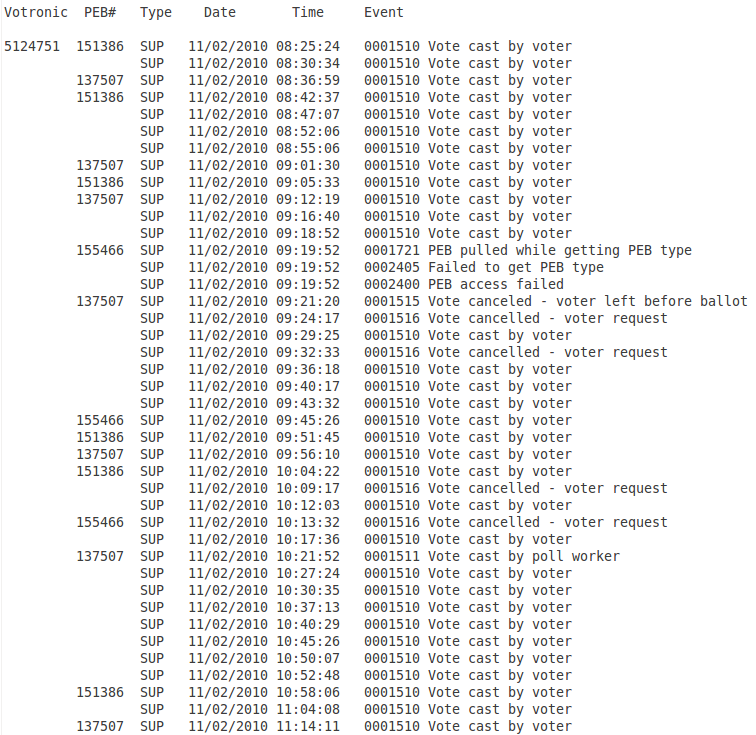
\includegraphics[width=0.8\textwidth]{eventLog}
%~\ref{app:el}

\clearpage
\section{Ballot Image File}\label{app:bi}
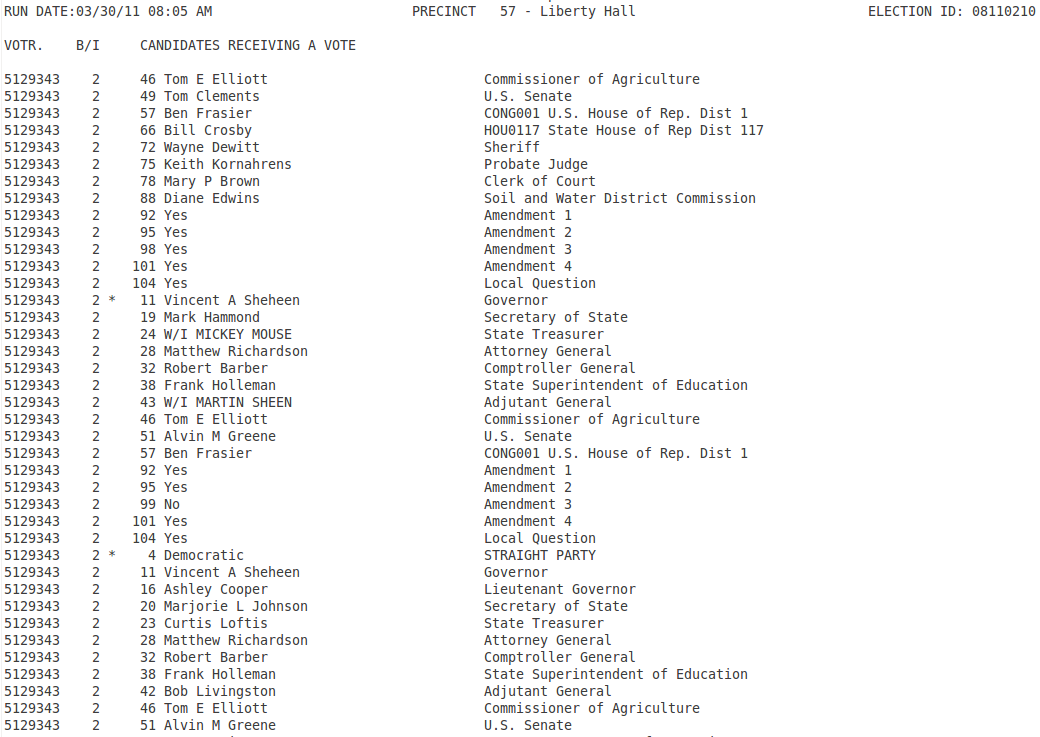
\includegraphics[width=0.9\textwidth]{ballot}
%This is app~\ref{app:bi}

\clearpage
\section{System Log File}\label{app:sl}
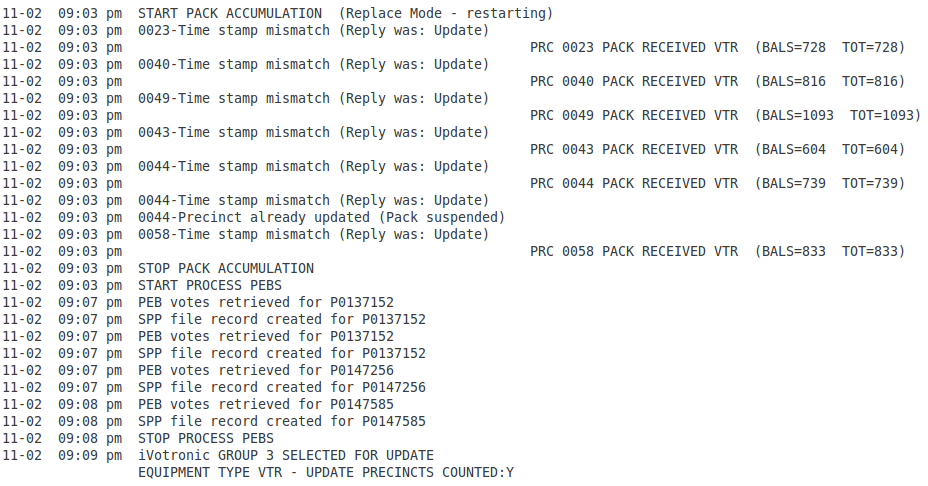
\includegraphics[width=0.9\textwidth]{system}
%This is app~\ref{app:sl}
\end{center}

\end{document}
